\chapter{Implementation}
\label{implementation}

% summary
In this chapter, the tools and techniques used in building this human-computer collaborative VR-based system are described. The focus will be on interaction techniques for different modes of operation. In addition, the setup of the robot and the construction of test scenes will also be covered in this chapter.


\section{Overview}
The main goal of this work is to design and implement a VR-based human-robot collaboration system with different methods of operating the robot in order to find out which method of operation is more suitable to be used to control the rescue robot. Further, it is to provide some basic insights for future development directions and to provide a general direction for finding an intuitive, easy-to-use and efficient operation method. Therefore, the proposed system was developed using Unity, including four modes of operation and a corresponding test environment for simulating post-disaster scenarios. In each operation mode, the user has a different method to control the robot. In addition, in order to better simulate the process by which the robot scans its surroundings and the computer side cumulatively gets a reconstructed 3D virtual scene, the test environment was implemented in such a way that the picture seen by the user depends on the direction of the robot's movement and the trajectory it travels through.


\section{System Architecture}
The proposed system runs on a computer with the Windows 10 operating system. This computer has been equipped with an Intel Core i7-8700K CPU, 32 GB RAM as well as a NVIDIA GTX 1080 GPU with 8 GB VRAM. HTC Vive is used as a VR device. It has a resolution of 1080 × 1200 per eye, resulting in a total resolution of 2160 × 1200 pixels, a refresh rate of 90 Hz, and a field of view of 110 degrees. It includes two motion controllers and uses two Lighthouses to track the position of the headset as well as the motion controllers.

Unity was chosen as the platform to develop the system. Unity is a widely used game engine with a Steam VR plugin \footnote{https://assetstore.unity.com/packages/tools/integration/steamvr-plugin-32647}, which allows developers to focus on the VR environment and interactive behaviors in programming, rather than specific controller buttons and headset positioning, making VR development much simpler. Another reason why Unity was chosen as a development platform was the potential for collaboration with the Robot Operating System (ROS), a frequently used operating system for robot simulation and manipulation, which is flexible, low-coupling, distributed, open source, and has a powerful and rich third-party feature set. In terms of collaboration between Unity and ROS, Siemens provides open source software libraries and tools in C\# for communicating with ROS from .NET applications \footnote{https://github.com/siemens/ros-sharp}. Combining ROS and Unity to develop a collaborative human-robot interaction platform proved to be feasible\cite{Whitney:2018wk}. Since the focus of this paper is on human-robot interaction, collaboration and synchronization of ROS will not be explored in detail here.

\section{Robot}
To simulate the process of a robot using a probe camera to detect the real environment and synchronise it to Unity, a conical collision body was set up on the robot. The robot will transform the Layers of the objects in the scene into visible Layers by collision detection and a trigger event (onTriggerEnter function). The robot's driving performance, such as the number of collisions, average speed, total distance, etc., will be recorded in each test. The detailed recorded information can be seen in Fig.\ref{fig:uml}. The movement of the robot depends on the value of the signal that is updated in each mode. In addition, the robot's Gameobject has the NavMeshAgent \footnote{https://docs.unity3d.com/ScriptReference/AI.NavMeshAgent.html} component, which supports the robot's navigation to the specified destination with automatic obstacle avoidance in the test scene. The virtual robot has three cameras. Each camera is set up in such a way that it can only see the area detected by the robot's radar and change the image bound to it in real time. The four operations described later all use the camera viewport as a monitoring screen by rendering the camera viewport on UI canvas.


\section{Interaction techniques}
This system has 4 different approaches to control the robot. Each mode has its own distinctive features: 

\begin{enumerate}
\item In Handle Mode the user will send control commands directly using the motion controller. 
\item In Lab Mode a simulated lab is constructed in the VR environment and the user will use virtual buttons in the lab to control the rescue robot. 
\item In Remote Mode the user can set the driving destination directly. 
\item In UI Mode the user has a virtual menu and sends commands via rays from the motion controller.
\end{enumerate}

In order to improve the reusability of the code and to facilitate the management of subsequent development, the classes that manage the interaction actions of each mode implement the same interface. A graphical representation of the system structure is given in the UML activity diagram in Fig.\ref{fig:uml}.

\begin{figure}[h]
    \centering
    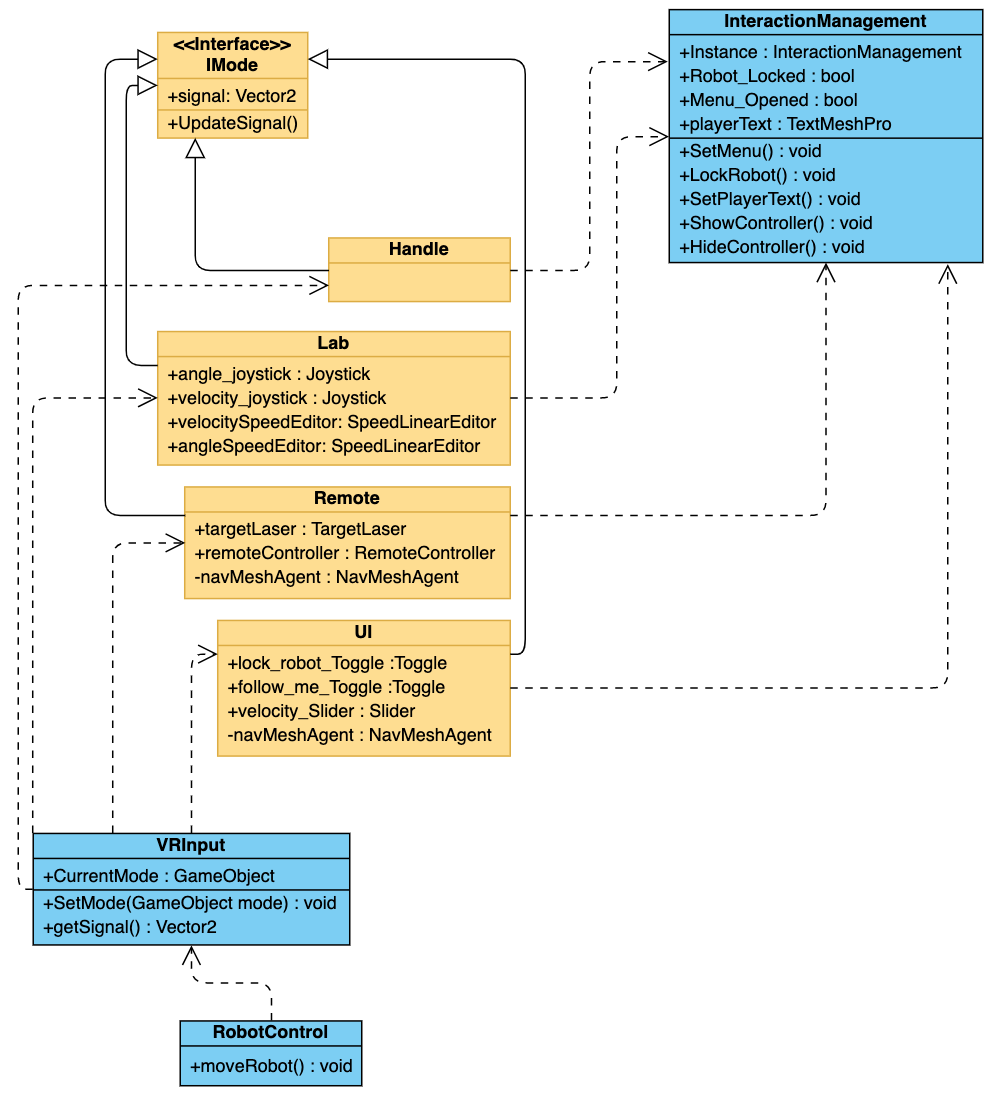
\includegraphics[height=12cm]{graphics/uml.png}
    \caption{UML Class diagram for the main structure of the system}
    \label{fig:uml}
\end{figure}

\subsection{Handle Mode}
\subsection{Lab Mode}
\subsection{Remote Mode}
\subsection{UI Mode}


\section{Test Scene}
In order to simulate the use of rescue robots in disaster scenarios, the test scenes were built to mimic the post-disaster urban environment as much as possible. The POLYGON Apocalypse\footnote{https://assetstore.unity.com/packages/3d/environments/urban/polygon-apocalypse-low-poly-3d-art-by-synty-154193}, available on the Unity Asset Store, is a low poly asset pack with a large number of models of buildings, streets, vehicles, etc. Using this resource pack as a base, additional collision bodies of the appropriate size were manually added to each building and obstacle after the pack was imported, which was needed to help track the robot's driving crash in subsequent tests.

Considering that there are four modes of operation to be tested, four scenes with similar complexity, similar composition of buildings but different road conditions and placement of buildings were constructed. The similarity in complexity of the scenes ensures that the difficulty of the four tests is basically identical. The different scene setups ensure that the scene information learned by the user after one test will not make him understand the next test scene and thus affect the accuracy of the test data. 

The entire scene is initially invisible, and the visibility of each objects in the test scene is gradually updated as the robot drives along. Ten interactable sufferer characters were placed in each test scene. The place of placement can be next to the car, the house side and some other reasonable places.
